\chapter{白矮星、中子星和强场物理}
\label{chap:11}

\begin{chapteropening}
白矮星和中子星把量子物理推到天文尺度。白矮星的半径由电子简并压、库仑修正和包层结构决定；中子星的光变由强引力、强磁场和相对论磁层共同投影到事件表上。可测量的仍是到达时间、能量、偏振和相位，只是这些量现在对应 \(10^6\) 到 \(10^{15}\,\mathrm{G}\) 的磁场、毫秒到小时的周期、以及 \(10\,\mathrm{km}\) 到地球半径量级的发光区域。
\end{chapteropening}

\section{白矮星：电子简并压怎样变成可测半径}

白矮星的主标度可由冷费米气体近似来理解。一个质量 \(M\simeq 0.6\,M_\odot\)、半径 \(R\simeq 0.012\,R_\odot\simeq 1.3\,R_\oplus\) 的典型 DA 白矮星，平均密度已经达到 \(10^6\,\mathrm{g\,cm^{-3}}\) 量级，中心密度可到 \(10^6-10^9\,\mathrm{g\,cm^{-3}}\)。在这种密度下，电子热运动只占次要地位；Pauli 不相容原理给电子填满动量空间，费米动量为
\begin{equation}
  p_F=\hbar (3\pi^2 n_e)^{1/3}, \qquad n_e=\frac{\rho}{\mu_e m_p}.
  \label{eq:ch11-01}
\end{equation}
\begin{formulaexplain}
\(p_F\) 是电子费米动量，\(n_e\) 是电子数密度；\(\rho\)、\(\mu_e\)、\(m_p\) 把质量密度换成电子数。它说明白矮星越密，电子被 Pauli 原理推到越高动量。
\end{formulaexplain}
这里 \(n_e\) 是电子数密度，单位 \(\mathrm{cm^{-3}}\)；\(\rho\) 是质量密度；\(m_p\) 是质子质量；\(\mu_e\) 是每个电子对应的重子数，碳氧白矮星通常取 \(\mu_e\simeq2\)。当 \(p_F\ll m_e c\) 时，电子非相对论，压强为
\begin{equation}
  P_{\rm NR}=\frac{(3\pi^2)^{2/3}}{5}\frac{\hbar^2}{m_e}n_e^{5/3};
  \label{eq:ch11-02}
\end{equation}
\begin{formulaexplain}
\(P_{\rm NR}\) 是非相对论电子简并压，随 \(n_e^{5/3}\) 增长。这个很硬的压强标度是普通白矮星能抵抗引力塌缩的主支撑。
\end{formulaexplain}
当 \(p_F\gtrsim m_e c\) 时，相对论效应把指数改成 \(4/3\)，
\begin{equation}
  P_{\rm ER}=\frac{(3\pi^2)^{1/3}}{4}\hbar c\, n_e^{4/3}.
  \label{eq:ch11-03}
\end{equation}
\begin{formulaexplain}
\(P_{\rm ER}\) 是极端相对论电子简并压，密度指数降为 \(4/3\)。支撑变软后，高质量白矮星半径会急剧缩小并接近极限质量。
\end{formulaexplain}
式中 \(P\) 的单位是 \(\mathrm{dyn\,cm^{-2}}\)。非相对论公式中，密度升高会迅速增加支撑压强；相对论公式中，高质量白矮星的支撑变得更软，质量继续增加时半径急剧变小，并走向 Chandrasekhar 极限 \citep{1931ApJ....74...81C,1935MNRAS..95..207C,1961ApJ...134..683H}。

实际写成观测者常用的质量半径近似，可用 Nauenberg 形式
\begin{equation}
  R\simeq 0.0112\,R_\odot
  \left[\left(\frac{M_{\rm Ch}}{M}\right)^{2/3}
  -\left(\frac{M}{M_{\rm Ch}}\right)^{2/3}\right]^{1/2},
  \qquad M_{\rm Ch}\simeq 5.83\,\mu_e^{-2}M_\odot .
  \label{eq:ch11-04}
\end{equation}
\begin{formulaexplain}
\(R\) 是白矮星半径，\(M\) 是质量，\(M_{\rm Ch}\) 是 Chandrasekhar 质量。质量越接近 \(M_{\rm Ch}\)，方括号越小，理想冷白矮星半径越小。
\end{formulaexplain}
这里 \(M_{\rm Ch}\) 是理想冷白矮星极限质量；对 \(\mu_e=2\)，\(M_{\rm Ch}\simeq1.46\,M_\odot\)。这个公式假设零温、非旋转、没有强磁场形变，适合用来估算 \(0.2-1.35\,M_\odot\) 白矮星的主标度。真实半径还受核心组成、氢氦包层厚度、有限温度和磁场影响，高精度工作需要演化模型或双星约束 \citep{1972ApJ...175..417N,2017MNRAS.470.4473P,2020ApJ...899..146C}。

\begin{figure}[tbp]
\centering
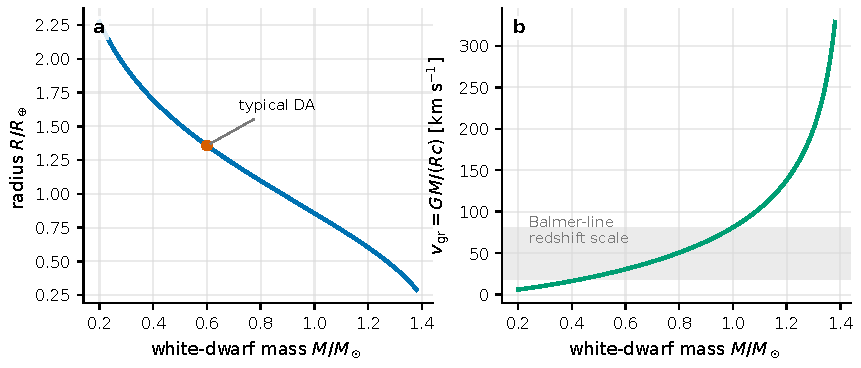
\includegraphics[width=0.94\linewidth]{figures/generated/chapter_11/ch11_white_dwarf_mass_radius.pdf}
\caption{白矮星质量增加时半径变小，靠近 Chandrasekhar 极限时收缩更快。右图把同一质量半径关系换成光谱中可测的引力红移速度 \(v_{\rm gr}=GM/(Rc)\)，典型 DA 白矮星的 Balmer 线红移是几十 \(\mathrm{km\,s^{-1}}\)，已经接近或超过普通恒星大气运动的速度尺度。}
\label{fig:chapter-11-wd-mr}
\end{figure}

质量半径关系可以通过几类数据进入观测。食双星的持续时间和径向速度给出 \(R/a\)、倾角和质量函数；视差加光谱能量分布可用 \(F_\lambda=(R/d)^2 H_\lambda(T_{\rm eff},\log g)\) 推出半径；谱线红移还能给出引力红移速度，
\begin{equation}
  v_{\rm gr}=\frac{GM}{Rc}
  \simeq 31.8\,\mathrm{km\,s^{-1}}
  \left(\frac{M}{0.6\,M_\odot}\right)
  \left(\frac{0.012\,R_\odot}{R}\right).
  \label{eq:ch11-05}
\end{equation}
\begin{formulaexplain}
\(v_{\rm gr}\) 是引力红移速度，正比于 \(M/R\)。谱线红移因此把白矮星质量半径关系变成可测速度，但必须扣除系统运动和线形成效应。
\end{formulaexplain}
这里 \(v_{\rm gr}\) 是谱线相对系统速度的红移。单个目标的系统速度、对流线移和 Stark 位移会污染这个量，所以大样本工作常把 Gaia 半径、SDSS 光谱线心和运动学模型一起平均。白矮星角直径本身很小，
\begin{equation}
  \theta_{\rm WD}=\frac{2R}{d}
  \simeq 11\,\mu{\rm as}
  \left(\frac{R}{0.012\,R_\odot}\right)
  \left(\frac{10\,{\rm pc}}{d}\right),
  \label{eq:ch11-06}
\end{equation}
\begin{formulaexplain}
\(\theta_{\rm WD}\) 是白矮星角直径，\(R\) 是半径，\(d\) 是距离。即使近到 \(10\,{\rm pc}\)，典型角尺度也只有微角秒，难以直接成像。
\end{formulaexplain}
所以即使在 \(10\,\mathrm{pc}\) 以内，普通光学成像也无法直接分辨。更可行的入口是把高速光度、偏振、谱线速度和相位信息保留在同一张事件表中。

\section{磁白矮星怎样把吸积几何写进相位和偏振}

磁白矮星把白矮星结构问题和光子统计问题连在一起。孤立磁白矮星的表面磁场可从 \(10^6\) 到 \(10^9\,\mathrm{G}\)，吸积系统中的极和中介极常见场强为 \(1-200\,\mathrm{MG}\)。磁矩写成
\begin{equation}
  \mu = B_* R_{\rm WD}^3
  \simeq 5.1\times10^{33}\,\mathrm{G\,cm^3}
  \left(\frac{B_*}{10\,{\rm MG}}\right)
  \left(\frac{R_{\rm WD}}{8\times10^8\,{\rm cm}}\right)^3 .
  \label{eq:ch11-07}
\end{equation}
\begin{formulaexplain}
\(\mu\) 是白矮星磁矩，\(B_*\) 是表面磁场，\(R_{\rm WD}\) 是半径。磁矩越大，磁场越能在更远处控制吸积流。
\end{formulaexplain}
这里 \(B_*\) 是白矮星表面磁场。给定 \(\mu\)、质量 \(M\) 和吸积率 \(\dot M\)，磁层半径的常用标度是
\begin{equation}
  r_m \simeq k
  \left(\frac{\mu^4}{2GM\dot M^2}\right)^{1/7},
  \label{eq:ch11-08}
\end{equation}
\begin{formulaexplain}
\(r_m\) 是磁层半径，\(k\) 是几何因子，\(\dot M\) 是吸积率。磁矩增强会推大磁层，吸积率升高会把磁层压向白矮星。
\end{formulaexplain}
其中 \(k\) 是几何因子，通常为 \(0.5-1\) 量级；\(\dot M\) 在激变变星中可从 \(10^{-11}\) 到 \(10^{-8}\,M_\odot\,{\rm yr^{-1}}\)。若 \(r_m\) 小于共转半径
\begin{equation}
  r_{\rm co}=\left(\frac{GM}{\Omega_s^2}\right)^{1/3},
  \label{eq:ch11-09}
\end{equation}
\begin{formulaexplain}
\(r_{\rm co}\) 是共转半径，\(\Omega_s\) 是白矮星自转角速度。在这个半径处，磁场共转角速度与 Kepler 轨道角速度相等。
\end{formulaexplain}
物质可以较顺利地沿磁力线落到磁极；若 \(r_m\) 接近或超过 \(r_{\rm co}\)，白矮星自转会把部分物质抛出或改变吸积流形态。中介极中 \(P_{\rm spin}/P_{\rm orb}\) 常在 \(0.01-0.6\)，极系统接近同步，\(P_{\rm spin}\simeq P_{\rm orb}\) \citep{1970ApJ...160L.147A,2000PASP..112..873W,1991MNRAS.249..460W,2008ApJ...672..524N}。

\begin{figure}[tbp]
\centering
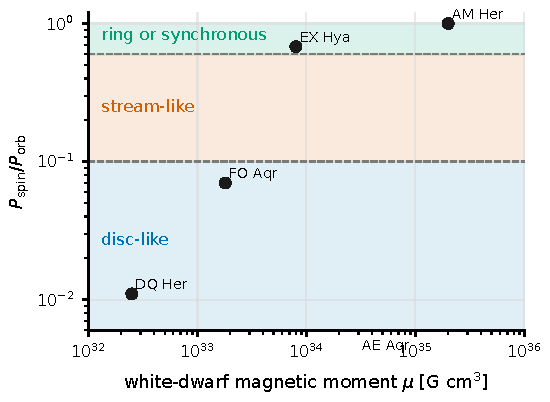
\includegraphics[width=0.78\linewidth]{figures/generated/chapter_11/ch11_magnetic_cv_flow_map.pdf}
\caption{磁激变变星的吸积流主要由白矮星磁矩和自转相对轨道的快慢决定。低 \(P_{\rm spin}/P_{\rm orb}\) 系统容易形成盘状流，中间区域常出现磁控流，接近同步或高比值系统会转向环状、流状或极系统几何；这些几何会直接改变光变相位、圆偏振和相关函数。}
\label{fig:chapter-11-mcv-map}
\end{figure}

吸积光度的数量级来自引力势能释放：
\begin{equation}
  L_{\rm acc}\simeq \frac{GM\dot M}{R_{\rm WD}}
  \simeq 1.0\times10^{33}\,\mathrm{erg\,s^{-1}}
  \left(\frac{M}{0.8\,M_\odot}\right)
  \left(\frac{\dot M}{10^{-10}M_\odot\,{\rm yr^{-1}}}\right)
  \left(\frac{8\times10^8\,{\rm cm}}{R_{\rm WD}}\right)
  \label{eq:ch11-10}
\end{equation}
\begin{formulaexplain}
\(L_{\rm acc}\) 是吸积光度，来自单位时间释放的引力势能。它给出磁激变变星可用光子率的数量级，实际光学只接收其中一部分。
\end{formulaexplain}
估算。光学波段只看到其中一部分，通常是盘、热斑、柱状冲击区、回照面和 cyclotron 辐射的混合。偏振能把 cyclotron 成分挑出来：圆偏振的符号随自转相位翻转时，通常表明视线穿过不同磁极或不同磁场投影；线偏振和总光变不同步时，强度峰和磁场几何峰往往不是同一个区域。

\Needspace{12\baselineskip}
事件表分析可以按自转相位或轨道相位分箱。令 \(\phi_s\) 是白矮星自转相位，\(I_{\phi_s}(t)\) 是该相位窗内的光子计数率，则
\begin{equation}
  g^{(2)}_{\phi_s}(\tau)=
  \frac{\langle I_{\phi_s}(t)I_{\phi_s}(t+\tau)\rangle}
  {\langle I_{\phi_s}(t)\rangle^2}
  \label{eq:ch11-11}
\end{equation}
\begin{formulaexplain}
\(g^{(2)}_{\phi_s}(\tau)\) 是固定自转相位窗内的二阶强度相关。它把同一磁极或吸积流片段在延迟 \(\tau\) 上的短时记忆提取出来。
\end{formulaexplain}
测的是同一个磁极或同一段吸积流在延迟 \(\tau\) 上的强度记忆。若 \(\tau\) 是毫秒到秒，信号可能来自冲击区冷却、磁控团块或探测器死时间；若 \(\tau\) 是几十秒到分钟，通常更像经典 flickering 或大气透明度变化。公式中的平均应在相同相位窗、相同能段和相同偏振通道内完成，否则轨道调制会被误认为短时相关。

\section{中子星怎样把磁层写进相位事件表}

中子星的半径只有 \(10-14\,\mathrm{km}\)，质量却常在 \(1.2-2.2\,M_\odot\)。自转把磁层切成相位坐标，最基本的长度是光柱半径
\begin{equation}
  R_{\rm LC}=\frac{c}{\Omega}=\frac{cP}{2\pi}
  \simeq 1.6\times10^3\,\mathrm{km}
  \left(\frac{P}{33\,{\rm ms}}\right).
  \label{eq:ch11-12}
\end{equation}
\begin{formulaexplain}
\(R_{\rm LC}\) 是光柱半径，\(P\) 是自转周期，\(\Omega\) 是角速度。它标出刚性共转达到光速的尺度，也是开放磁力线的基本边界。
\end{formulaexplain}
这里 \(P\) 是自转周期，Crab 脉冲星 \(P\simeq33\,\mathrm{ms}\)，毫秒脉冲星 \(P\simeq1.5-10\,\mathrm{ms}\)，磁星常为 \(2-12\,\mathrm{s}\)。在 \(R_{\rm LC}\) 之外，刚性共转需要超过光速，所以开放磁力线、粒子加速和高能辐射都要在这个尺度内组织。脉冲星发现和旋转中子星解释确立了这套图像，Crab 又把旋转能损失和超新星遗迹联系在一起 \citep{1968Natur.217..709H,1968Natur.218..731G,1968Natur.219..145P,1972ApJ...175..217B}。

\begin{figure}[tbp]
\centering
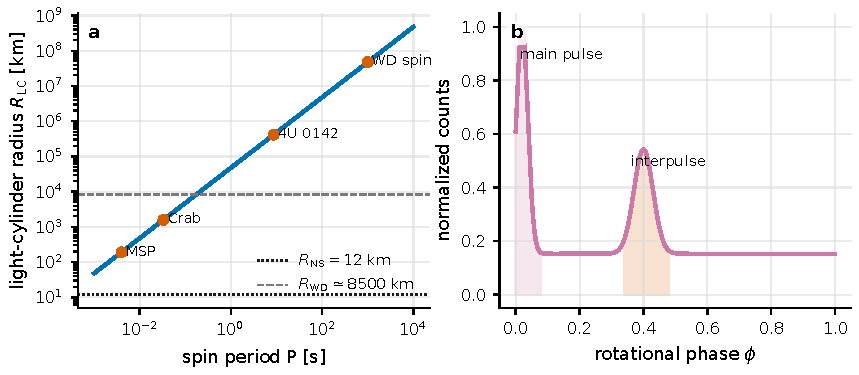
\includegraphics[width=0.94\linewidth]{figures/generated/chapter_11/ch11_light_cylinder_phase.pdf}
\caption{光柱半径随自转周期线性增加。毫秒脉冲星的光柱只有几十到几百公里，Crab 约 \(1.6\times10^3\,\mathrm{km}\)，磁星则可到 \(10^5\,\mathrm{km}\) 以上。右图是 Crab 型相位折叠轮廓，主脉冲和 interpulse 的相位窗决定哪些光子进入后续的强度相关或偏振统计。}
\label{fig:chapter-11-light-cylinder}
\end{figure}

磁偶极估算给表面赤道场
\begin{equation}
  B_{\rm dip}\simeq 3.2\times10^{19}(P\dot P)^{1/2}\,\mathrm{G},
  \label{eq:ch11-13}
\end{equation}
\begin{formulaexplain}
\(B_{\rm dip}\) 是由自转慢化估算的偶极磁场，\(P\) 和 \(\dot P\) 来自计时。它把事件到达时间中的慢化率换成磁场标度。
\end{formulaexplain}
\Needspace{12\baselineskip}
其中 \(P\) 用秒，\(\dot P\) 是无量纲的 \(\mathrm{s\,s^{-1}}\)。普通年轻脉冲星常在 \(10^{11}-10^{13}\,\mathrm{G}\)，磁星可到 \(10^{14}-10^{15}\,\mathrm{G}\)。旋转能损失率写成
\begin{equation}
  \dot E = 4\pi^2 I\frac{\dot P}{P^3},
  \qquad I\simeq10^{45}\,\mathrm{g\,cm^2}.
  \label{eq:ch11-14}
\end{equation}
\begin{formulaexplain}
\(\dot E\) 是自转能损失率，\(I\) 是转动惯量。它衡量脉冲星可用于驱动磁层辐射和星云的能量预算。
\end{formulaexplain}
Crab 的 \(\dot E\) 是 \(10^{38}\,\mathrm{erg\,s^{-1}}\) 量级，足以驱动从射电到 \(\gamma\) 射线的脉冲和星云辐射 \citep{1984ApJ...283..279H,1992ApJ...397..187B,2001A&A...378..918K,2008ApJ...680.1378H}。

事件表进入脉冲星分析时，每个光子先做太阳系质心改正，再用时序星历折叠：
\begin{equation}
  \phi_i =
  \left[
  \nu(t_i-t_0)+\frac{1}{2}\dot\nu(t_i-t_0)^2
  +\frac{1}{6}\ddot\nu(t_i-t_0)^3+\cdots
  \right]\bmod 1 .
  \label{eq:ch11-15}
\end{equation}
\begin{formulaexplain}
\(\phi_i\) 是第 \(i\) 个光子的自转相位，\(\nu,\dot\nu,\ddot\nu\) 是频率及其导数。这个折叠式把到达时间表变成相位事件表。
\end{formulaexplain}
这里 \(t_i\) 是第 \(i\) 个光子的质心到达时刻，单位秒；\(\nu=1/P\) 是自转频率；\(\dot\nu\) 和 \(\ddot\nu\) 描述慢化和 glitch 后恢复。Crab 的主脉冲宽度约占相位 \(0.04-0.05\)，射电巨脉冲可窄到微秒量级。若把巨射电脉冲发生的周期挑出来，光学主脉冲平均会增强约 \(3\%\)，而脉冲形状和到达相位基本不变；ARCONS 的能量分辨光子计数进一步显示，早到的巨射电脉冲对应的光学增强可达十几到二十几个百分点 \citep{2003Sci...301..493S,2013ApJ...779L..12S}。这些结果把相干射电爆发和非相干光学辐射接到同一部分磁层等离子体上。

相位分辨二阶相关可写为
\begin{equation}
  g^{(2)}_{ab}(\tau|\Phi)=
  \frac{\langle n_a(t,\Phi)n_b(t+\tau,\Phi)\rangle}
  {\langle n_a(t,\Phi)\rangle\langle n_b(t,\Phi)\rangle},
  \label{eq:ch11-16}
\end{equation}
\begin{formulaexplain}
\(g^{(2)}_{ab}(\tau|\Phi)\) 是相位窗 \(\Phi\) 内两个通道 \(a,b\) 的相关。它可比较不同能段、偏振或望远镜在同一脉冲相位的同步涨落。
\end{formulaexplain}
其中 \(a,b\) 可以是能段、偏振通道或不同望远镜，\(\Phi\) 是主脉冲、bridge 或 interpulse 相位窗。对 Crab 这样的亮目标，\(\tau\) 可以推进到微秒至毫秒；对更暗的光学脉冲星，最先能做的通常是相位窗内的光度和偏振堆叠，离单脉冲统计还有距离 \citep{1996ApJ...468..779M,2000ApJ...537..861S,2009MNRAS.397..103S}。

\section{强磁场偏振怎样检验传播中的量子效应}

强磁场偏振的基本标尺是 QED 临界场
\begin{equation}
  B_Q=\frac{m_e^2c^3}{e\hbar}
  =4.414\times10^{13}\,\mathrm{G}.
  \label{eq:ch11-17}
\end{equation}
\begin{formulaexplain}
\(B_Q\) 是 QED 临界磁场，在这个场强下电子回旋能量接近静能。磁星表面磁场接近或超过它，真空传播不再像普通介质外的空白背景。
\end{formulaexplain}
当 \(B\ll B_Q\) 且光子能量远低于 \(m_ec^2\) 时，Heisenberg-Euler 有效理论给真空折射率差的弱场近似
\begin{equation}
  \Delta n \simeq
  \frac{\alpha_{\rm fs}}{30\pi}
  \left(\frac{B_\perp}{B_Q}\right)^2 ,
  \label{eq:ch11-18}
\end{equation}
\begin{formulaexplain}
\(\Delta n\) 是两个偏振正常模的折射率差，\(B_\perp\) 是横向磁场。弱场近似显示双折射效应随 \(B_\perp^2\) 快速增强。
\end{formulaexplain}
\Needspace{13\baselineskip}
其中 \(B_\perp\) 是垂直于光线方向的磁场分量，\(\alpha_{\rm fs}\) 是精细结构常数。磁星表面 \(B\sim10^{14}-10^{15}\,\mathrm{G}\)，弱场公式不能直接当作精确模型，但它给出偏振对强场敏感的原因：两个正常模的相位差沿路径积累，
\begin{equation}
  \Delta \Phi(E)=\frac{E}{\hbar c}\int \Delta n(s)\,ds .
  \label{eq:ch11-19}
\end{equation}
\begin{formulaexplain}
\(\Delta\Phi(E)\) 是两个偏振模积累的相位差，\(E\) 是光子能量。能量越高、路径上 \(\Delta n\) 越大，偏振传播效应越明显。
\end{formulaexplain}
这里 \(E\) 是光子能量，X 射线偏振仪常在 \(2-8\,\mathrm{keV}\) 工作；积分沿光路进行。若传播是绝热的，偏振矢量会随局部磁场方向转动，直到偏振限制半径之后冻结。这个物理图像来自强场 QED、磁层传播和中子星表面辐射模型的组合 \citep{1936ZPhy...98..714H,1971AnPhy..67..599A,2000MNRAS.311..555H,2002PhRvD..66b3002H,2003MNRAS.342..134H}。

\Needspace{12\baselineskip}
偏振观测需要同时报告强度、偏振度和偏振角。线偏振的事件估计通常从调制角 \(\eta_i\) 出发，
\begin{equation}
  I=\sum_i w_i,\qquad
  Q=\sum_i w_i\cos 2\eta_i,\qquad
  U=\sum_i w_i\sin 2\eta_i,
  \label{eq:ch11-20}
\end{equation}
\begin{formulaexplain}
\(I,Q,U\) 是 Stokes 量，\(\eta_i\) 是单个事件的调制角，\(w_i\) 是权重。偏振仪把许多光子的方位角累加成线偏振信号。
\end{formulaexplain}
然后得到
\begin{equation}
  p=\frac{\sqrt{Q^2+U^2}}{I},\qquad
  \psi=\frac{1}{2}\arctan2(U,Q).
  \label{eq:ch11-21}
\end{equation}
\begin{formulaexplain}
\(p\) 是线偏振度，\(\psi\) 是偏振角。\(Q,U\) 的矢量长度给偏振强度，方向给天空上的偏振角。
\end{formulaexplain}
这里 \(p\) 是线偏振度，取值 \(0-1\)；\(\psi\) 是偏振角；\(w_i\) 包含仪器调制因子、背景权重和有效面积权重。光学偏振测量 RX J1856.5-3754 得到 \(p=16.43\%\pm5.26\%\)，源本身 \(V\simeq25.5\)，前景偏振和仪器偏振都要逐项扣除；这类测量和热表面模型相比，支持真空双折射会减少不同表面区域的偏振相消 \citep{2015MNRAS.454.3254T,2016MNRAS.459.3585G,2017MNRAS.465..492M}。

\begin{figure}[tbp]
\centering
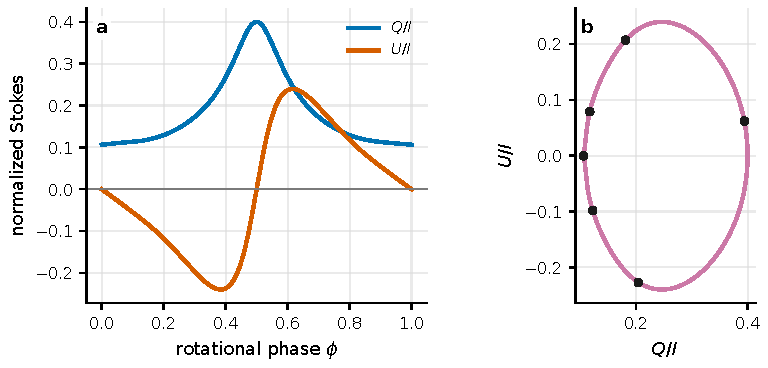
\includegraphics[width=0.92\linewidth]{figures/generated/chapter_11/ch11_stokes_qu_track.pdf}
\caption{旋转磁几何会把偏振角变化投影成 \(Q/I\) 和 \(U/I\) 的相位曲线。左图显示同一相位事件表给出的两个 Stokes 分量，右图显示对应的 Q-U 轨迹；轨迹形状比单独的偏振度更能暴露几何退化和仪器串扰。}
\label{fig:chapter-11-stokes}
\end{figure}

相位依赖的偏振角常用旋转矢量模型作第一近似：
\begin{equation}
  \tan(\psi-\psi_0)=
  \frac{\sin\alpha \sin(\phi-\phi_0)}
  {\sin\zeta\cos\alpha-\cos\zeta\sin\alpha\cos(\phi-\phi_0)} .
  \label{eq:ch11-22}
\end{equation}
\begin{formulaexplain}
\(\psi\) 是偏振角，\(\alpha\) 是磁轴倾角，\(\zeta\) 是视线倾角，\(\phi\) 是自转相位。旋转矢量模型把相位上的偏振角摆动翻译成磁层几何。
\end{formulaexplain}
这里 \(\alpha\) 是磁轴和自转轴夹角，\(\zeta\) 是视线和自转轴夹角，\(\phi\) 是自转相位，\(\psi_0\) 和 \(\phi_0\) 是零点。这个公式最早用于射电脉冲星偏振几何；在磁星 X 射线中，它只是低维几何骨架，因为表面辐射、共振 cyclotron 散射和真空双折射会一起改变 \(p(E,\phi)\) 和 \(\psi(E,\phi)\) \citep{1969ApL.....3..225R,2018ApJ...854...98W,2011ApJ...730..131F}。

\begin{figure}[tbp]
\centering
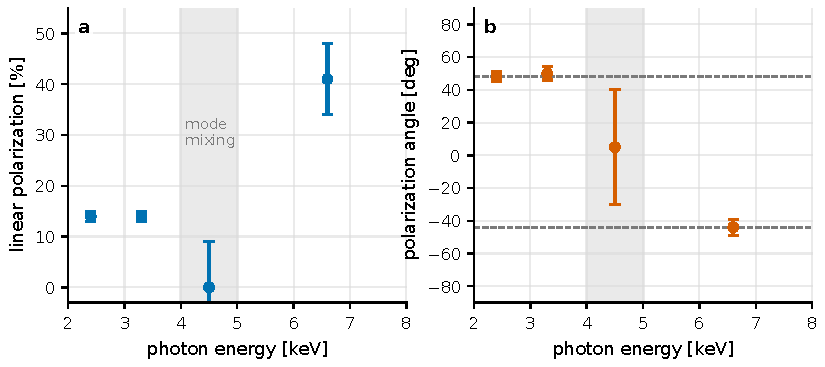
\includegraphics[width=0.92\linewidth]{figures/generated/chapter_11/ch11_birefringence_energy.pdf}
\caption{IXPE 对磁星 4U 0142+61 的结果可以看成两个偏振正常模在能量上的切换。低能 \(2-4\,\mathrm{keV}\) 偏振度约 \(14\%\)，高能 \(5.5-8\,\mathrm{keV}\) 升到约 \(41\%\)，而 \(4-5\,\mathrm{keV}\) 附近偏振度接近最低可探测偏振，偏振角发生约 \(90^\circ\) 翻转。}
\label{fig:chapter-11-birefringence}
\end{figure}

4U 0142+61 是一个具体例子。IXPE 在 \(2-8\,\mathrm{keV}\) 看到总线偏振度 \(12\%\pm1\%\)，低能 \(2-4\,\mathrm{keV}\) 为 \(14\%\pm1\%\)，高能 \(5.5-8\,\mathrm{keV}\) 为 \(41\%\pm7\%\)，中间 \(4-5\,\mathrm{keV}\) 附近偏振度降到灵敏度附近并伴随偏振角约 \(90^\circ\) 翻转。源的自转周期 \(P=8.69\,\mathrm{s}\)，磁场 \(B\sim10^{14}\,\mathrm{G}\)，软 X 射线有 \(kT\sim0.5-1\,\mathrm{keV}\) 黑体成分，硬尾可延伸到几十甚至上百 keV。解释这组数据时，低能 O 模、硬尾 X 模、表面凝聚态或薄大气、以及共振 Compton 散射都可能参与；单个高偏振点还不足以单独构成真空双折射探测 \citep{2022Sci...378..646T,2023A&A...674L..10C,2023MNRAS.519.3681F}。

\section{热斑光变怎样反推中子星半径}

中子星半径不能直接量角直径，只能从光变形状、能谱和相对论传播反推。紧致度
\begin{equation}
  u=\frac{2GM}{Rc^2}
  \simeq 0.345
  \left(\frac{M}{1.4\,M_\odot}\right)
  \left(\frac{12\,{\rm km}}{R}\right)
  \label{eq:ch11-23}
\end{equation}
\begin{formulaexplain}
\(u\) 是中子星紧致度，等于 Schwarzschild 半径与真实半径之比。\(u\) 越大，引力光弯曲越强，热斑光变振幅越容易被抹平。
\end{formulaexplain}
决定光弯曲强度。\(u\) 越大，背面热斑越容易被弯到视线中，脉冲振幅越小、轮廓越平滑。一个常用近似把发射角 \(\alpha\) 和斑点相对视线的中心角 \(\psi\) 联系起来：
\begin{equation}
  \cos\alpha \simeq u+(1-u)\cos\psi .
  \label{eq:ch11-24}
\end{equation}
\begin{formulaexplain}
\(\alpha\) 是光子离开表面时的发射角，\(\psi\) 是斑点中心相对视线的角距。这个近似把弯曲后的可见性写成紧致度的简单函数。
\end{formulaexplain}
它适用于 Schwarzschild 外部时空、慢自转或中等自转的标度估算；快速毫秒脉冲星还要加入 Doppler boost、像差、时延、星体扁率和大气束射 \citep{2002ApJ...566L..85B,2019AIPC.2127b0008W}。

\begin{figure}[tbp]
\centering
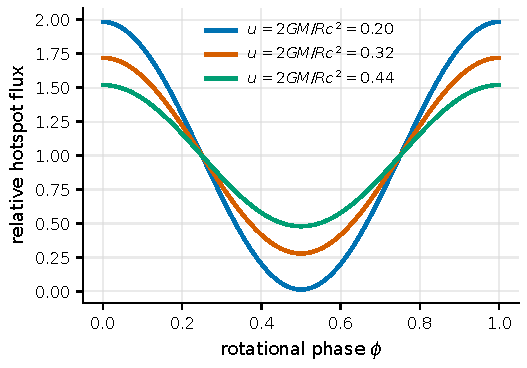
\includegraphics[width=0.78\linewidth]{figures/generated/chapter_11/ch11_hotspot_lightcurve.pdf}
\caption{热斑光变对紧致度很敏感。低紧致度时，斑点转到背面后贡献迅速消失，脉冲振幅大；高紧致度时，引力光弯曲让更大范围的表面可见，光变谷底被抬高。半径推断利用这种轮廓变化，并与质量、倾角、热斑位置和大气束射一起拟合。}
\label{fig:chapter-11-hotspot}
\end{figure}

对一个带能谱的热斑，探测器中第 \(j\) 个能道、第 \(k\) 个相位 bin 的期望计数可写成
\begin{equation}
  \lambda_{jk}(\Theta)=
  T\int dE\,
  R_j(E)\,
  \left[
  F_E(\phi_k;\Theta)+B_E
  \right].
  \label{eq:ch11-25}
\end{equation}
\begin{formulaexplain}
\(\lambda_{jk}\) 是能道 \(j\)、相位 bin \(k\) 的期望计数，\(R_j(E)\) 是仪器响应，\(F_E\) 是热斑模型通量。它把天体模型变成探测器中的预期事件数。
\end{formulaexplain}
\Needspace{13\baselineskip}
这里 \(T\) 是曝光时间，\(R_j(E)\) 是有效面积和能量重分布组成的响应，\(F_E\) 是模型热斑通量，\(B_E\) 是背景，\(\Theta\) 包含 \(M,R\)、距离、倾角、斑点经纬度、斑点角半径、温度和大气参数。实际计数服从 Poisson 统计：
\begin{equation}
  \ln{\cal L}(\Theta)=
  \sum_{j,k}\left[
  N_{jk}\ln\lambda_{jk}(\Theta)-\lambda_{jk}(\Theta)-\ln(N_{jk}!)
  \right].
  \label{eq:ch11-26}
\end{equation}
\begin{formulaexplain}
\(\ln{\cal L}\) 是 Poisson 对数似然，\(N_{jk}\) 是观测计数。半径推断就是寻找让所有能道和相位 bin 的 \(\lambda_{jk}\) 最接近事件表的参数 \(\Theta\)。
\end{formulaexplain}
NICER 对 PSR J0030+0451 和 PSR J0740+6620 的半径结果属于这种事件表建模。J0740 的分析把 NICER 事件表、XMM-Newton 成像光谱背景、以及射电计时给出的质量和距离先验联合起来；Riley 等得到 \(R=12.39^{+1.30}_{-0.98}\,\mathrm{km}\)、\(M=2.072^{+0.067}_{-0.066}M_\odot\)，Miller 等得到相容但方法不同的半径约束。J0030 的两套独立分析也显示，热斑几何可能包含复杂的多极磁场结构 \citep{2019ApJ...887L..21R,2019ApJ...887L..24M,2021ApJ...918L..27R,2021ApJ...918L..28M}。

